% First release on June 21, 2010
% Modified on Dec 12, 2017 by XSK

\documentclass[twoside,twocolumn]{article}
\def\@oddhead{\mbox{}\scriptsize\rightmark \hfil \thepage}%
\usepackage{fitee}
\usepackage{tabularx, multirow}
\usepackage{graphicx,subfigure}
%\usepackage[colorlinks, breaklinks = true]{hyperref}		% for pdflatex
\usepackage[dvips, hidelinks, breaklinks = true]{hyperref}  % for DVI to PDF latex
\addto{\captionsenglish}{%
  \renewcommand{\figurename}{Fig.}
}

\begin{document}

%% article title
\title{Improving Neighbor Discovery with Slot Index Synchronization}

%% when all authors provide emails, no $\dagger$
\author[$\dagger$$\ddagger$1]{Shuai-zhao JIN}%
\author[$$2]{Zi-xiao WANG}%
\author[$$2]{Ben Leong}%
\author[$$1]{Ya-bo Dong}%
\author[$$1]{Dong-ming Lu}
\affil[1]{School of Computer Science and Technology of Zhejiang University, Hangzhou 310027, China}
\affil[2]{Department of Computer Science, National University of Singapore, Singapore}

\shortauthor{Jin et al.}	% one author: only Zhai; two authors: Zhai and Hu; three authors: Zhai et al.

\authmark{}

%% Only 1 affiliations
%\author{Wen-fei WANG}
%\author{Rong XIONG$^{\dagger\ddagger}$}
%\author{Jian CHU}
%\affil{\it\footnotesize State Key Laboratory of Industrial Control Technology, Institute of Cyber-Systems and Control,
%	\authorcr\it\footnotesize Zhejiang University, Hangzhou 310027, China}

% for authors, use \authorcr to begin with a new line, e.g., \author[2]{\authorcr Xian-liang HU}
% for the affiliation, use \authorcr\Affilfont\it to begin with a new line, e.g.,
%\affil[1]{Editorial Office of Journal of Zhejiang University SCIENCE,
%\authorcr\Affilfont\it Hangzhou 310027, China}

\corremailA{jinszhao@zju.edu.cn} 
%\corremailB{xlhu@zju.edu.cn}
%\corremailC{abc@zju.edu.cn}
%\corremailD{ABC@zju.edu.cn}
\emailmark{$\dagger$}	% when all authors provide emails, no \dagger


% abbrev. of month: Jan. Feb. Mar. Apr. May June July Aug. Sept. Oct. Nov. Dec.
\dateinfo{Received mmm.\ dd, 2016;	Revision accepted mmm.\ dd, 2016;    Crosschecked mmm.\ dd, 2017}


\abstract{Neighbor discovery is essential for \emph{docking} applications, where mobile nodes communicate with
static nodes situated at various rendezvous points. In existing neighbor discovery protocols, the probabilistic
protocols perform well in the average-case but have aperiodic, unpredictable and unbounded discovery latency.
While the deterministic protocols can provide a bounded worst-case discovery latency, they achieve this by
sacrificing the average-case performance. In this paper, we propose a new synchronization technique, called
Mobility-Assisted Slot index Synchronization (MASS). MASS improves the average-case performance of deterministic
neighbor discovery protocols via \emph{slot index synchronization}, without incurring additional energy consumption.
We evaluate MASS through both theoretical analysis and simualtions of the real traces from a tourist tracking system
deployed at Mogao Grottoes, a famous cultural heritage site in China. We show that MASS can reduce the average
discovery latency of state-of-the-art deterministic neighbor discovery protocols by up to 2 orders of magnitude.
}
% separate by semicolons 
\keywords{Neighbor discovery; Docking applications, Slot index synchronization; MASS}


\doi{10.1631/FITEE.1000000}	% DOI of the paper, should be accurate
\code{A}
\clc{TP}

%\inpress	% uncomment this command if use "in press"

\publishyear{2018}
\vol{19}
\issue{1}
\pagestart{1}
\pageend{5}

%% when no funding, the following line should be removed, no period at last
\support{Project supported by the National High Technology Research and Development Program of China (No.2012AA101701) and
the National Key Technology Support Program of China (No.2013BAK01B00, No.2014BAK16B00)} 

%\conf{A preliminary version of this paper has been presented at ??? Conference, date}
%\esm{Electronic supplementary materials: The online version of this article (http://dx/doi.org/10.1631/jzus.C1000000) contains supplementary materials, which are available to authorized users}
\orcid{Shuai-zhao JIN, http://orcid.org/0000-0002-5176-5607}	% corresponding author, or first author
\articleType{}
%\articleType can be `Science Letters:', `Review:', `Comment:', etc.
%Leave blank for research article.

\maketitle



\section{Introduction} 
\label{sec:introduction}
The availability of cheap wireless sensor networks has made \emph{docking applications}~\citep{Dutta2008Practical} 
feasible for widespread deployment. In docking applications, there are two sets of sensor nodes: static and mobile
nodes. Static nodes are placed at fixed rendezvous points and mobile nodes are attached to moving objects of interest.
Some examples of docking applications include the uploading of cargo transit history~\citep{malinowski2007cargonet}, 
the tracking of cattle movement during feeding times~\citep{wark2007model}, the tracking of hikers via their encounters 
with trail-sid waypoints~\citep{huang2005cenwits} and our application, which tracks tourists at a cultural heritage 
site~\citep{ming2008wireless}.

For the conservation work in Mogao Grottoes, a famous cultural heritage site in China, it is essential to track and 
study how the movement of tourists around the caves affects the micro-climate in caves. The current tracking system
in place consists of static ndoes placed in the caves and mobile nodes carried by the tour guides. The static nodes
emit beacons which are picked up by the mobile nodes for each tour group that enters a cave. Not only is the 
detection of the tour group important, it is also essential to accurately measure the duration of stay within each
cave. In addition, power is also a constraint for the tracking system as modern infrastructure is not allowed to be
installed in the caves to supply power to the static nodes.

In the current tracking system, the static nodes are configured at a duty cycle of 0.6\%~(they wake up and send beacons
for 30~ms every 5~s) and the mobile nodes are always active and continuously listen for the beacons. While this achieves
an average discovery latency of 2.5~s, the mobile nodes have to be charged daily, which is inconvenient and is also a
major impediment to our plans for scaling up the system. Our goal is to reduce energy consumption by introducing duty
cycling for the mobile nodes, without compromising discovery latency.

Neighbor discovery protocols will allow both the static and mobile nodes to duty cycle while ensuring discovery. Through
different wake-sleep patterns design, neighbor discovery protocols ensure that nodes will wake up within the same time
slot to discover each other. Our key insight is that \emph{discovery latency can be minimized by synchronizing the active 
and sleeping slots of the nodes}. This is because when the slot indices are synchronized, the nodes will discover each 
other at the next earliest active slot, i.e., the next overlapping active slot.

While this might sound straightforward, it turns out that synchronizing the nodes for a docking application introduces
a number of challenges. First, the synchronization must be done in a distributed manner as the static nodes cannot 
directly communicate with each other. Instead, they can only communicate by using the mobile nodes to relay information.
Second, the synchronization should converge quickly in order to achieve any gains. Finally, the intrinsic inaccuracies
in the clocks of the sensors will result in \emph{clock drift}. If the synchronization of the slots drifts by a small
amount, the resulting latency could potentially become the worst case, instead of being optimal. In other words, 
synchronization could significantly degrade performance instead of improving performance if we are not careful.

We propose and evaluate Mobility-Assisted Slot index Synchronization~(MASS), which improves the average-case performance
of existing deterministic neighbor discovery protocols via \emph{slot index synchronization}. In MASS, the nodes first
elect a reference node in a distributed manner and then synchronize their slot indices with that reference node. We
exploited the natural visiting patterns of tourists to elect the reference node. For our Mogao Grottoes traces, MASS is
able to synchronize all the 60 static nodes within three hours, which is less than half of the 10-hour operational period
of the site. But even if it is not able to synchronize all the nodes, we can still reduce the discovery latency for the
nodes that are synchronized. To mitigate the impact of the clock drift, MASS employs existing techniques to estimate the 
clock skew between the nodes and compensate for the clock drift with respect to the elected reference node. The experiments
show that our sensor nodes can achieve the error of 0.98~ms and 2.4~ms per hour for 50\% and 90\% of the time, respectively,
which is well within one slot interval.

We evaluate MASS via simulation using a real 31-day trace obtained from the existing Mogao Grottoes tourist tracking system
and show that MASS can reduce the discovery latency of 4 existing deterministic protocols~(BlindDate~\citep{wang13blinddate}, 
Searchlight~\citep{bakht2012searchlight}, Disco~\citep{Dutta2008Practical} and U-Connect~\citep{kandhalu2010u}) by about 2 
orders of magnitude over 75\% of the time. Therefore, with MASS, we are able to achieve a discovery latency of less than 5~s
for 70\% of the time, even when the duty cycle of the nodes is reduced to 0.5\% to save power. By reducing the duty cycle
from 100\% to 0.5\%, our mobile nodes will be able to last 200 tiems longer and be charged every 6 months instead of daily.

To the best of our knowledge, we are the first to propose the use of slot index synchronization to improve neighbor discovery
latency in docking applications. We addressed the resulting challenges by utilizing existing techniques such as clock skew
estimation and clock drift compensation, and proposing a synchronization process and priority metric. It remains as future
work to thoroughly investigate how MASS performs on practical sensor networks, especially on the tourist tracking system
deployed at the Mogao Grottoes.

The rest of the paper is organized as follows: in Section~\ref{sec:related}, we present an overview of existing neighbor 
discovery protocols as well as clock synchronization and drift compensation techniques. In Section~\ref{sec:challenge}, 
we describe our docking application scenario, our key insight and explain the challenges for our system. In Section, we 
describe the MASS algorithm. We evaluate MASS in Section and conclude in Section.

\section{Related Work}
\label{sec:related}

{\bf Neighbor Discovery Protocols.} Neighbor discovery protocols are needed in duty-cycled 
networks to ensure discovery. Most neighbor discovery protocols are \emph{slotted} protocls
and divide time into identically-sized discrete slots. In each slot, sensor nodes either
sleep or wake up according to some pattern determined by the protocol. Existing protocols
can be classified by their adoption of either \emph{probabilistic} or \emph{deterministic}
wake-sleep slot schedules to achieve an overlap. In probabilistic protocols, the sleep-wake 
schedule is based on some randomized function~\citep{mcglynn2001birthday}. With the right
parameters, probabilistic protocols can achieve good average-case performance. Unfortunately, 
the worst-case performance is unbounded, i.e., there is a small chance that two nodes will 
never discover each other.

On the other hand, deterministic protocols provide a bounded worst-case latency as the sleep-wake 
schedule is designed to ensure discovery within one sleep-wake period. Prime-based protocols such 
as Disco~\citep{Dutta2008Practical} and U-Connect~\citep{kandhalu2010u} guarantee a bounded discovery 
latency based on the Chinese Remainder Theorem~\citep{niven2008introduction}. Quorum-based 
deterministic protocols~\citep{tseng2003power,lai2010heterogenous} have slots that are grouped into 
a 2-dimensional $m \times m$ array for a period of $m^2$.  Each node picks one row and one column 
of the entries as its active slots, thus ensuring that any two nodes will have at least two overlapping 
active slots in each period. The state-of-the-art Searchlight~\citep{bakht2012searchlight} protocol 
further reduces the overlapping slots to at least one by grouping the slots into an array of size 
$\lfloor\frac{m}{2}\rfloor \times m$. The duty cycle can be further reduced by {\em striped probing}, 
where the probe skips every two slots. Extending the duration of the active slots ensures overlap
and guarantees detection.  BlindDate~\citep{wang13blinddate} is a recently proposed protocol to 
improve the performance of Searchlight by having two dynamic probe slots traversing towards each other 
in opposite directions within each period. BlindDate also requires the extension of active slots like 
Searchlight.  Sun et al.\ proposed Hello~\citep{sun14hello}, a generalized framework for deterministic
protocols that can represent existing protocols such as Quorum, Disco, U-Connect and Searchlight, using 
a set of parameters.  They proved that Searchlight is the optimal symmetric protocol.  Our technique,
MASS, complements existing deterministic protocols and can significantly reduce discovery latency 
through slot index synchronization.

{\bf Clock Synchronization.} There are two common approaches for clock synchronization in multihop 
wireless networks~\citep{sun14survey}: (i) reference-based clock synchronization; and (ii) distributed 
clock synchronization. In reference-based clock synchronization, the nodes synchronize their clocks 
with respect to one or more reference nodes. These reference nodes are known as roots in tree-based
protocols~\citep{su2005time,ganeriwal2003timing}, gateways in cluster-based protocols~\citep{elson2002fine}, 
and time servers in NTP-based protocols~\citep{ye2008dtp}. The main drawback of reference-based protocols 
is that they are not robust to the failures of reference nodes. Furthermore, they all assume that a 
reliable means of communication exists between the nodes.  This assumption does not hold for our tourist 
tracking system.

In distributed clock synchronization, all nodes run the same distributed synchronization algorithm, which 
will cause their local clocks to converge to a common global time value.  Some techniques to achieve global 
synchronization include having each node advance its clock to the fastest clock~\citep{jiang2004clock,zhou2007accurate}, 
or to the average clock values of the local nodes~\citep{li2006global,sommer2009gradient,sasabe2009simple}.  
Glossy is a recent network flooding architecture that achieves an average time synchronization error below 
one microsecond~\citep{ferrari11glossy}.  However, it is not suitable in docking applications because the 
mobile nodes are not always connected.  To cope with frequent topology changes and long inter-contact duration, 
Choi et al.\ developed distributed asynchronous clock synchronization (DCS) for delay tolerant networks~\citep{choi2012dcs}.  
Global clock synchronization is achieved by asynchronously compensating for clock errors using relative clock
information exchanged among nodes in DCS. The drawback of distributed synchronization algorithms is that 
convergence is slow (it typically takes hundreds of iterations)~\citep{he12random}. Furthermore, such
protocols only work well in a closed system, where no new nodes join the network once it starts.

\section{A Case for Slot Index Synchronization}
\label{sec:challenge}
In this section, we introduce the background for our target docking application system, 
and show that slot index synchronization is a promising technique to improve the 
performance of deterministic neighbor discovery protocols. We also explain why distributed
synchronization algorithms are not feasible for our application.

\subsection{Tourist Tracking in Historical Sites}

\begin{figure}[t]
  \centering 
  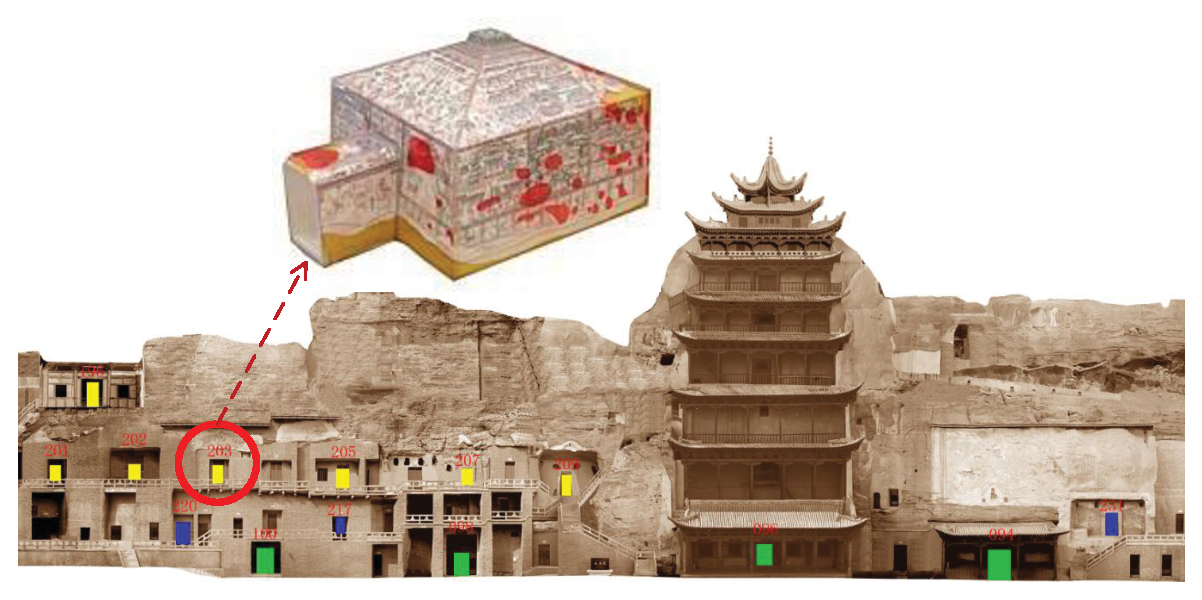
\includegraphics[scale=0.35]{static/mogao}
  \caption{Mogao Grottoes}
  \label{fig:mogao}
\end{figure}

Mogao Grottoes, also known as the Caves of the Thousand Buddhas, is a
famous cultural heritage site in China. It consists of hundreds of
caves cut into the side of a cliff, some of which have Buddhist murals
painted all over the walls and ceilings.  Fig.~\ref{fig:mogao} shows
a small section of the Mogao Grottoes. Thousands of tourists visit the
Mogao Grottoes every day, and the high volume of human traffic will
change the micro-climate in caves which may cause deterioration to the 
priceless historical artwork. Therefore, it is important to monitor and 
limit the number of visitors to each cave to mitigate the over-exposure 
of the artwork due to human contact.

The challenge of tracking tourists in such a historical site is that
modern infrastructure such as power supply lines cannot be installed. 
Neither are fixtures allowed to be drilled into the walls
for fear of damaging the cultural artefacts. The current tracking
system deployed uses static low-power sensor nodes placed at the
corners of the caves which periodically emit beacon signals.  Each
tour guide holds a mobile sensor node that continuously listens for
and logs these beacons as the tour group visits each cave.  At the end
of the tour, the durations of the stay for each tour group in the
caves is extracted and recorded from the mobile nodes.

The tourist tracking system is an example of a {\em docking}
application. As the cave walls block the radio signals, static nodes
cannot communicate with each other directly. It is also not feasible
to deploy more nodes to create a fully connected wireless sensor
network due to conservation restrictions on the number of nodes that
can be deployed.

The lack of power infrastructure also means that static nodes have to
be powered by battery, which implies that energy consumption is a very
important consideration. To reduce energy consumption, the static
nodes currently perform duty cycle where they spend 30\,ms every 5\,s
listening and broadcasting beacons.  On the other hand, the mobile
nodes have to be continuously listening to detect static nodes as well
as record the entering and leaving time of tourists, thereby requiring
daily battery recharging. Considering hundreds of mobile nodes in use,
daily battery recharing is a huge impediment to scale up our tracking
system.

Neighbor discovery protocols provide a way to allow both the static and 
mobile nodes to duty cycle and thus reducing energy consumption. However, 
it is at the cost of increased discovery latency. The {\em discovery latency} 
is determined by the neighbor discovery protocol and the duty cycle rate 
determines the trade-off between discovery latency and energy consumption. 
In our case, it is equally important to also measure the accurate duration 
of stay for tourists in the caves to monitor the environmental effects of 
human traffic which impose a great need for small discovery latency.

\subsection{Slot Index Synchronization}

\begin{figure}[t]
   \centering
   \includegraphics[width=.9\columnwidth]{figs/disco_example}
   \caption{Disco with a pair of primes (3, 5)} 
   \label{fig:disco_example}
\end{figure}

Probabilistic neighbor discovery protocols like Birthday~\citep{mcglynn2001birthday} 
have lower average-case discovery latencies, but the worst-case latency 
is unbounded. Deterministic protocols like Disco~\citep{Dutta2008Practical} 
and Searchlight~\citep{bakht2012searchlight} have slightly higher average 
discovery latencies but bounded worst-case latencies. Our key observation 
is that {\em slot index synchronization has a significant impact on the 
discovery latency for deterministic protocols}.

To illustrate this, Fig.~\ref{fig:disco_example} shows the discovery
process between three nodes that run Disco with the parameters (3, 5).
This gives a duty cycle of about 50\% and a period of 15 slots.  The
shaded and white boxes represent active and sleeping slots
respectively.  In this example, node A and B are strictly
synchronized, and node C is out-of-sync by one slot. Suppose all three
nodes come into contact at time $t_1$, node A and B will discover each
other at time $t_2$ with a latency of two slots, while node C will
discover the rest at time $t_3$ with a latency of five slots. It is
clear from this illustration that when the nodes are synchronized, the
worst-case latency is the largest gap between the active slots.

To investigate the improvement that can be achieved with synchronized
nodes, we enumerated all possible slot offsets between a pair of nodes
running the same symmetric protocol, and recorded the discovery
latency as the number of slots it takes from first contact to the
first intersecting active slot for the two nodes. We treated adjacent
active slots as a successful detection as well, because perfect
alignment rarely exists in real life and partially overlapping slots
are sufficient for detection. This is especially important for
BlindDate and Searchlight-S (Searchlight with striped probing) because
perfect alignment may cause failure of detection. To overcome this,
these protocols extend the active slot so as to ensure overlap of
adjacent active slots.


We computed the distribution of the discovery latency of the different
protocols with duty cycles of 5\% and
1\%~\citep{wang13blinddate, sun14hello, bakht2012searchlight}, and plot
the result for 5\% duty cycle in Fig.~\ref{fig:latency-cdf}. The
result for 1\% duty cycle is similar. Our analysis shows that, with
the same duty cycle, Searchlight-S is the best performing protocol
with the lowest average-case and worst-case latency.

\begin{figure}[t]
   \centering
   \includegraphics{graphs/analysis/latency-cdf}
   \caption{Cumulative distribution of discovery latency for the
		          various protocols at duty cycle of 5\%.}
   \label{fig:latency-cdf}
\end{figure}


\begin{table*}[t]\footnotesize
   \centering
   \caption{Average and worst-case discovery latency. Values in
		        brackets indicate the latency in seconds.}
     %\vspace{-6pt}
   \label{tab:latency}
   \begin{tabularx}{\textwidth}{@{}l *{7}{>{\centering\arraybackslash}X} @{}}
      \toprule
      & \multicolumn{2}{c}{{\em Overall Performance}} & \multicolumn{2}{c}{{\em Synchronized Index}} & \multirow{3}{\linewidth}[-2em]{\centering Average Latency Improvement} & \multirow{3}{\linewidth}[-2em]{\centering Worst-case Latency Improvement} & \multirow{3}{\linewidth}[-2em]{\centering Parameter(s)} \\
      \cmidrule[.5pt](r){2-3}
      \cmidrule[.5pt](l){4-5}
      Protocol & Average Latency & Worst-case Latency & Average Latency & Worst-case Latency  \\
      & (slots)[s]  & (slots)[s] & (slots)[s] & (slots)[s] \\
      \cmidrule(lr){2-2}
      \cmidrule(lr){3-3}
      \cmidrule(lr){4-4}
      \cmidrule(lr){5-5}
      & \multicolumn{7}{c}{\bf\scriptsize 5\% Duty-cycle, 25\,ms per slot} \\[-2pt]
      \cmidrule[.5pt](l){2-8}
      Searchlight-S   & 151 [3.78] & 399 [9.98] & 12.3 [0.31] & 37 [0.93] & 12.28 & 10.78 & 40\\
      BlindDate       & 168 [4.20] & 685 [17.13] & 13.8 [0.35] & 46 [1.15] & 12.17 & 14.89 & 12\\
      Disco           & 194 [4.85] & 1,071 [26.78] & 12.7 [0.32] & 36 [0.90] & 15.28 & 29.75 & (37, 43)\\
      U-Connect       & 423 [10.6] & 960 [24.00] & 14.6 [0.37] & 30 [0.75] & 28.97 & 32.00 & 31\\
									    
      & \multicolumn{7}{c}{\bf\scriptsize 1\% Duty-cycle, 5\,ms per slot} \\[-2pt]
      \cmidrule[.5pt](l){2-8}
      Searchlight-S   & 4,711 [23.56] & 9,999 [50.00]  & 65.7 [0.33] & 197 [0.99] & 71.70 & 50.76 & 200\\
      BlindDate       & 6,387 [31.94] & 17,821 [89.11]  & 71.4 [0.36] & 238 [1.19] & 89.45 & 74.88 & 60\\
      Disco           & 10,125 [50.63] & 35,655 [178.28] & 64.1 [0.32] & 180 [0.90] & 157.96  & 198.08  & (181, 211)\\
      U-Connect       & 11,123 [55.62] & 22,800 [114.00] & 74.6 [0.37] & 150 [0.75] & 149.10  & 152.00  & 151\\
      \bottomrule
  \end{tabularx}
\end{table*}

We also compared the average-case and worst-case latency of each
protocol against the case where both nodes have their slot indices
synchronized in Table~\ref{tab:latency}.  The key observation is that
the average and worst-case latency are significantly lower when the
nodes are synchronized on their slot indices. This result is intuitive
since two synchronized nodes follow the same sleep-wake pattern and
thus wake up at the same time.  What is surprising is the amount of
improvement. Even for the best performing protocol, Searchlight-S at
1\% duty cycle, the average latency is reduced by 72 times.  With the
slot size of 5\,ms, we can reduce the average latency from 24\,s to
0.33\,s, and the worst-case latency from 50\,s down to about 1\,s.

While slot index synchronization improves performance greatly, we
cannot always guarantee the synchronization between two nodes due to
the inherent errors in the sensor hardware. For example, the timing
signals are produced by electronic components, known as oscillators.
The oscillation frequency may vary due to different reasons such as
the temperature and vibration which is known as \emph{clock skew}.
Hence, the effectiveness of slot synchronization is dependent on the 
accuracy of synchronization.


\subsection{Distributed Synchronization Not Feasible}

In a docking application, static nodes are not able to communicate
with each other directly and have to rely on mobile nodes to relay
information. One approach to achieve synchronization would be to use a
distributed clock synchronization algorithm such as DCS~\citep{choi2012dcs}.  
The duty cycle of the nodes can then be derived from the resulting 
reference clock, and synchronizing their clocks will naturally 
synchronize the slot indices.

However, this approach does not work for two reasons. First, we have
found that DCS either fails or takes an extremely long time to
synchronize the clocks of nodes to within an accuracy of one slot
duration.  This means that either node indices will never be
synchronized, or the improvement would be small due to the long
convergence time.  Second, DCS is designed to work in a closed system,
where no nodes leave or join the system. Otherwise, it can no longer
guarantee convergence.  In our docking application, the mobile nodes
can leave and new mobile nodes may enter the system at any time.

Because of the shortcomings of the distributed algorithms, we adopt a
reference-based technique for synchronization, where a node is elected
to be the reference node that all other nodes synchronize with.  Our
key observation is that although the mobile nodes do not follow a
pre-determined path, the movement is not completely random.  Thus, we
exploited the movement pattern of tourists and designed a simple
algorithm to elect the reference node.

\section{Mobility-Assisted Slot Synchronization}
\label{sec:mass}

We have shown that slot index synchronization can significantly
improve latency. In this section, we describe the design of
Mobility-Assisted Slot index Synchronization (MASS) for our tourist
tracking application at Mogao Grottoes.

Since static nodes cannot directly communicate with each other, mobile
nodes are used to relay information between the static nodes.  The
challenge is that mobile nodes do not move along pre-determined
paths. Thus, we cannot determine prima facie which static node will be
visited next.  However, we observed from the traces of our real-world
application that the paths of the mobile nodes tend to follow a
certain set of patterns. We can exploit the patterns to elect
relatively stable reference nodes in a distributed manner, and have
the non-reference nodes synchronize their slot index with these
reference nodes. In addition, we use the clock of the reference node
as the reference clock for clock drift compensation.

All static and mobile nodes will adopt the same neighbor-discovery
protocol with a common set of parameters. Thus, if all (or most) of
the static nodes have their slot indices synchronized, mobile nodes
can likewise have their slot indices synchronized with every static
node. This results in a very small discovery latency when they come
into contact with any of the synchronized static nodes.

\subsection{Distributed Reference Election \& Synchronization}
\label{sec:selection}

%\begin{figure}[t]
%   \centering
%   \begin{subfigure}[b]{\columnwidth}
%       \centering
%       \includegraphics[scale=0.35]{figs/illustration-1}
%   \end{subfigure}
%      \parbox{.8\columnwidth}
%      {\smallskip\scriptsize
%      Mobile node $m$ has no initial reference. Static node $r$ also
%      has no reference while static node $s$ has previously
%      synced with node $p$.\\}
%  \begin{subfigure}[b]{\columnwidth}
%      \centering
%      \includegraphics[scale=0.35]{figs/illustration-2}
%  \end{subfigure}
%      \parbox{.8\columnwidth}
%      {\smallskip\scriptsize
%      Node $m$ encounters node $r$, synchronizes with $r$ and
%      updates its reference to $P_r$.\\}
%  \begin{subfigure}[b]{\columnwidth}
%      \centering
%      \includegraphics[scale=0.35]{figs/illustration-3}
%  \end{subfigure}
%      \parbox{.8\columnwidth}
%      {\smallskip\scriptsize
%      Now $m$ leaves and encounters node $s$. Suppose $P_r'<P_s'$
%      and $P_s'<P_p$, node $m$ syncs with node $s$ and updates its
%      reference to $P_p$.\\}
%  \begin{subfigure}[b]{\columnwidth}
%      \centering
%      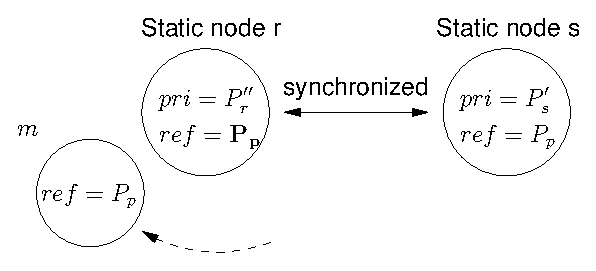
\includegraphics[scale=0.35]{figs/illustration-4}
%  \end{subfigure}
%      \parbox{.8\columnwidth}
%      {\smallskip\scriptsize
%      Suppose now $m$ returns to node $r$, and suppose even after
%      updating $P_r''$, $P_r''<P_p$, then node $r$ will sync with $m$
%      and record $P_p$ as its reference. Now nodes $r$ and $s$ will be
%      in sync.\\}
%\caption{Reference node election.} 
%\label{fig:selection}
%\end{figure}

\begin{table}[t]
   \centering
   \caption{Summary of update rules for reference node election}
      %\vspace{-6pt}
   \begin{tabularx}{\columnwidth}{@{}Xll@{}}
     \toprule
     Condition & Static node & Mobile node \\
     \midrule
     $P_{m} > P_{s}$ and $P_{m} > P_{s.ref}$ & $P_{s.ref} \leftarrow P_m$ & No Change \\
     $P_{m} < P_{s}$ or $P_{m} < P_{s.ref}$ & No Change & $P_m \leftarrow \textrm{max}(P_s, P_{s.ref})$ \\
     \bottomrule
   \end{tabularx}
   \label{tab:priority}
\end{table}

To elect the reference nodes, we introduce the notion of a priority
metric $P$.  Each static node $s$ computes a priority $P_s$ based on
information carried by the mobile nodes in a distributed way. In
addition, each static node $s$ also stores the recorded priority of
its reference, $P_{s.ref}$ obtained from the mobile nodes. Similarly,
each mobile node, $m$, also stores the priority ($P_m$) of the last
static node that it is synchronized with. When a mobile node $m$
encounters a new static node $s$, the static node first updates its
priority $P_s$. Then, the priorities $P_s$, $P_{s.ref}$, and $P_m$ are
compared and exchanged.

If $P_m$ is larger than $P_s$ and $P_{s.ref}$, then the static node
will synchronize its clock and slot index according to that of the
mobile node, and set its reference $P_{s.ref}$ to $P_m$. Indirectly,
the static node will have now synchronized with the static node that
the mobile node has last synchronized with. On the other hand, if
$P_m$ is smaller than $P_s$ or $P_{s.ref}$, the mobile node will
synchronize its slot index with the static node.  It will also
set its reference $P_m$ to the larger of $P_s$ and $P_{s.ref}$.
Figure~\ref{fig:selection} illustrates the steps of this process and
Table~\ref{tab:priority} summarizes the above update rules. With this
simple algorithm, the node with the largest priority value will be
elected as the reference node, from which other nodes will take
reference.  It remains for us to describe how a static node $s$
determines and computes its priority $P_s$.

\begin{figure}[t]
   \centering
   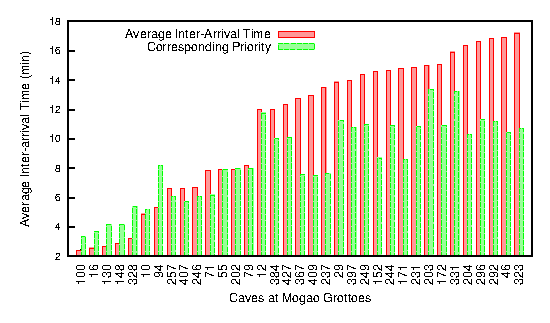
\includegraphics[scale=0.7]{graphs/visiting_frequency/visitingfrequency}
   \caption{Average inter-arrival time and the priority of different
            caves at Mogao Grottoes for day one.}
   \label{fig:visitingfrequency}
\end{figure}

{\bf Node Priority}. For our reference node election algorithm to work
well, not only does the priority $P_s$ need to be a metric that can be
easily computed in a distributed way, the resulting priority for
different static nodes should also preferably be distinct. In our
docking application, we observed that some caves were more popular
than others due to either its intrinsic attractiveness to the
tourists, or its relative location, i.e., it might be near route
entrances. Such caves will have more visitors than others. Thus, we
decided to utilize the average inter-arrival time between mobile nodes
at each static node $s$ to obtain its priority $P_s$.

The static nodes compute $P$ by measuring the time elapsed since the
last visit to the cave. The priority is accumulated using an
exponentially-weighted moving average (EWMA) with a smoothing factor
$\alpha = \frac{1}{8}$.  In other words, the equation to update $P_i$
to $P_{i+1}$ is:
\begin{equation}\label{eq1}
	P_{i+1} = \alpha t + (1 - \alpha) P_i
\end{equation}
where $t$ is the elapsed time since the last visit to this cave.

In Fig.~\ref{fig:visitingfrequency}, we plot the actual average
inter-arrival time of each cave over one day of a real trace and the
computed priority $P_i$.  Although the computed priority is often not
close to the actual daily average values, the trends are similar,
i.e., the more frequently visited nodes will have a higher priority.

It is entirely plausible that for some docking applications, the
static nodes have similar visiting frequencies and the computed
priorities might be very close to one another. In such cases, the
inter-arrival time might not be the best metric and another metric
could be used. However, our reference election algorithm is still
applicable if a good metric can be found.

\subsection{Clock Drift Compensation \& Slot Synchronization}

Once a reference node is elected, each node will synchronize their
clocks to that reference node. However, clock drift will introduce
errors, even if a node is perfectly synchronized at the start.  Hence,
both static and mobile nodes in our system must continuously estimate
and compensate for clock drift.

{\bf Clock Skew Estimation.}  There are many existing algorithms for
clock skew detection and
estimation~\citep{hamilton2008aces,yang2010adaptive,liao2013distributed}.
Zhong et al.\ showed that it is possible to continuously detect and
estimate the clock skew between two nodes~\citep{zhong2011demand}.  We
believe that any of the state-of-the-art techniques could be used for
MASS. For validation, we performed a simple experiment: a sensor node
periodically sends beacons at different intervals to three sensor
nodes that keep listening to compute relative clock skew, using the
following formula~\citep{huang2013psr, xu2013taco}:
\[
	\delta_{AB} = \frac{(t^A_{i+1} - t^A_i) - (t^B_{i+1} - t^B_i)}
	{t^A_{i+1} - t^A_i}
\]
where $t^A_i$ and $t^B_i$ are the local time at the sender's and
receiver's clock when the $i$th beacon was sent and received. The
MAC-layer time-stamping technique was used to mitigate the variance of
the delivery time~\citep{maroti2004flooding}.

%\begin{figure}[t]
%   \centering
%   \begin{subfigure}[b]{.32\textwidth}
%      \centering
%      \includegraphics{graphs/clock_skew_measure/skew_interval}
%      \caption{Mean and variance of clock skew measured at one node using different
%        time intervals.}
%      \label{fig:skew_int}
%   \end{subfigure}\hfill%
%   \begin{minipage}[b]{.32\textwidth}
%      \centering
%      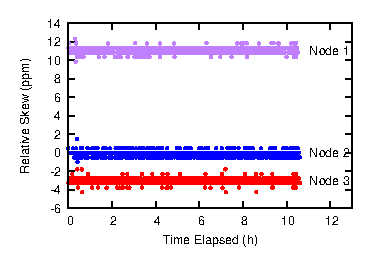
\includegraphics{graphs/clock_skew_measure/fournodes_skew_1minute}
%      \caption{Clock skew measured at 1-min intervals between the sending node
%        receiving nodes.}
%      \label{fig:skew_minute}
%   \end{minipage}\hfill%
%   \begin{minipage}[b]{.32\textwidth}
%      \centering
%      \includegraphics{graphs/clock-drift-experiment/cdc}
%      \caption{Amount of clock drift between two nodes with and without clock drift compensation.}
%      \label{fig:skew_cdc}
%   \end{minipage}
%   \caption{Clock skew of the three receiving nodes.}
%   \label{fig:skew}
%\end{figure}



\section{Paper format}

\subsection{Preparing manuscript}

The electronic manuscript should be prepared to accord with the following (see also http://www.zju.edu.cn/jzus/manuscript.htm):

\noindent \textbf{Title and by-line:} Name, affiliation (institution) of the author(s), city, zip code, country, and e-mail address of the author(s) should be given.

\noindent \textbf{Abstract:} About 150--250 words should outline the objective, method, main results, and conclusions without mathematical equations or citations.

\noindent \textbf{Key words:} Provide 3--6 key words or phrases for cross-indexing this article.

\noindent \textbf{Text:} The text should contain an Introduction that puts the paper into proper perspective for the reader, and should also contain Methods, Results, Discussion, and Conclusions sections.

\noindent \textbf{Acknowledgements:} Individuals or units other than authors who were of direct help in the work should be acknowledged by a brief statement following the text.

\noindent \textbf{References:} Only essential references (journal article, book, thesis, report, proceedings, etc.) cited in the text (in Author-Year format) can be listed in alphabetical order by author's surname.


\subsection{Revision \& acceptance}

\subsubsection{Figures}\label{sec:figure}

\noindent \textbf{Format:} At the revision stage, authors who have created their files using a drawing or painting program such as Visio, Origin, Excel, AutoCAD, Coreldraw should provide the original files that can be edited. Authors who have created their files using a drawing or painting program should export the files to TIFF, EPS, PSD, RAW, etc. format. Matlab figures are expected to be exported to EMF or EPS format. The figure's magnification should be expressed by scale bars.

\noindent \textbf{Resolution:} Adequate figure resolution is essential to a high-quality print and online rendering of your paper. Raster line art should carry an absolute minimum resolution of 600 dots per inch (dpi).

\noindent \textbf{Line width:} The line width should generally be no less than 0.25 pt; the common line widths are 0.5/0.75 pt. Please note that the actual line width changes with the scale of the figure. In different software, we recommend the following line widths: Visio: -- 03; Origin: -- 1.5; Matlab: -- 1.5 pt, etc.

Figures must be numbered consecutively with Arabic numerals, and each figure must be placed in the text following the paragraph in which it is first mentioned. A caption giving the figure number and a brief description must be included. The caption should be understandable without reference to the text. Figures should be cited in the text using the following format: Fig.~1, Fig.~1a, Figs.~1 and 2, Figs.~1--3, or Figs.~1a--1c.

There will be an extra charge for those graphics considered for publication in color. Authors are expected to use different line types to distinguish the different parts of a figure that they do not want to have published in color.

\begin{figure}[!htb]\small
\centering
\begin{tabular}{c}
\includegraphics[scale=0.9]{pics/jzusalogo.eps}\\
{\footnotesize\sf (a)} \\[3mm]
\includegraphics[scale=0.9]{pics/jzusblogo.eps}\\
{\footnotesize\sf (b)} \\
\includegraphics[scale=0.26]{pics/fiteelogo.eps}\\
{\footnotesize\sf (c)} \\
\end{tabular}
\caption{Logos of \emph{Journal of Zhejiang University-SCIENCE A (Applied Physics {\sf \slshape \&} Engineering)} (a), \emph{Journal of Zhejiang University-SCIENCE B (Biomedicine {\sf \slshape \&} Biotechnology)} (b), and \emph{Frontiers of Information Technology {\sf \slshape \&} Electronic Engineering} (c)}
\label{fig:logo}
\end{figure}


\begin{figure}[tbh]
	\centering
	\includegraphics[scale=0.60]{pics/outlierdetection.eps}
	\caption{Comparison of different methods in terms of outlier detection accuracy \citep{Zhou11}} \label{fig:Prediction}
\end{figure}


\subsubsection{Tables}\label{sec:table}

Tables should usually contain three horizontal lines. Do not use vertical lines. Each table must have a brief title that describes its contents. The title should be understandable without reference to the text. Details such as explanatory material, specific entries, and definitions of non-standard abbreviations should be put in table footnotes, not in the title. In setting up tables, authors should keep in mind the area of the Journal's page (16.4 cm $\times$ 22.8 cm) and the column width (8.0 cm) and should make tables conform to the limitations of these dimensions.

\begin{table*}[thp]\footnotesize
\centering
\caption{Results for face and eye detection processing using a Pentium IV 2.2 GHz CPU$^\textbf{*}$ \citep{Deniz10}} \label{Table:FacesDetected}
\addtolength{\tabcolsep}{4.8pt}
\begin{tabular*}{16.4cm}{lcccccccc}
	\toprule[0.75pt]
	\multirow{2}{*}{Detector}                  & \multicolumn{3}{c}{TD (\%)}  &  & \multicolumn{3}{c}{FD (\%)}  & \multicolumn{1}{c}{Processing time} \\
	\cmidrule[0.5pt]{2-4}\cmidrule[0.5pt]{6-8} & Faces & Left eye & Right eye &  & Faces & Left eye & Right eye &                (ms)                 \\ 
	\midrule[0.5pt]
	Rowley                                     & 89.27 &  77.51   &   78.18   &  & 2.16  &   0.80   &   1.00    &                422.4                \\
	Viola-Jones                                & 97.69 &   0.00   &   0.00    &  & 8.25  &          &           &                117.5                \\
	ENCARA2                                    & 99.92 &  91.83   &   92.48   &  & 8.07  &   4.04   &   3.33    &                45.6                 \\ 
	\bottomrule[0.75pt]
	\multicolumn{9}{p{15.6cm}}{\scriptsize $^*$ Taken from Castrill\'{o}n {et al}. (2007). TD: correct detection ratio; FD: false detection ratio}
\end{tabular*}
\end{table*}


All tables must be mentioned in the text in consecutive order and must be numbered with Arabic numbers. Tables should be cited in the text using the following format: Table~1, Tables~1 and 2, or Tables~1--3.


\begin{table}[thp]\footnotesize
\centering
\caption{Video sequences used in the experiments, ordered by increasing head motion$^\textbf{*}$ \citep{Deniz10}} \label{Table:1}
\addtolength{\tabcolsep}{4.8pt}
\begin{tabular*}{7.95cm}{cccc}
	\toprule[0.75pt]
	 Video   & Number of &  Average   &                   Variance                   \\
	sequence &  frames   &  distance  &                   position                   \\ 
	\midrule[0.5pt]
	   1     &    126    & 42.7 (1.6) &                     8.2                      \\
	   2     &    175    & 42.9 (2.2) &                     11.1                     \\
	   3     &    176    & 44.1 (1.8) &                     11.3                     \\
	   4     &    148    & 40.0 (2.8) &                     27.1                     \\
	   5     &    119    & 42.9 (2.8) &                     37.7                     \\
	   6     &    129    & 42.9 (4.4) &                    120.8                     \\
	   7     &    208    & 41.6 (3.1) &                    164.4                     \\ 
	\bottomrule[0.75pt]
	\multicolumn{4}{p{6cm}}{\scriptsize $^*$ Taken from images captured by camera 1}
\end{tabular*}
\end{table}

\subsubsection{Variables and formulate}

Variables, regardless of the context (formula, figure, or table), should be in Italics (e.g., $x_1$); if a variable represents a vector or a matrix, it should be in Italics \& Bold (e.g., $\bm{x}_1$). Numerals and operators should never be italicized unless they are components of a variable. The following are some typical equations \citep{Theodoridis11}:

\begin{equation}
\frac{\mathrm{d}}{\mathrm{d}t} {| \bar{\bm{x}}_{f_i} \cdot {\bm{W}}_{f_i}^l |^2 }= ({{\bm{W}}_{f_i}^l})^\mathrm{T} \dot {\bm{W}}_{f_i}^l \bar {\bm{x}}_{f_i} ({\bar {\bm{x}}_{f_i}})^\mathrm{T},
\end{equation}
\begin{equation}\label{indicatorfunc}
I_{j_1, j_2, \ldots, j_n}^{l_1, l_2, \ldots, l_n} (\bm{x}(t))= 
	\begin{cases}
		\alpha(\bm{x}(t)), & \mathrm{if}\ \bm{x}(t) \in \Omega_{j_1, j_2, \ldots, j_n}^{l_1, l_2, \ldots, l_n}, \\
		0,                 & \mathrm{otherwise},
	\end{cases}
\end{equation}
\begin{equation}\label{eqn:Lyapdisturb1}
\begin{aligned}
	\dot{V} & \leq  - \lambda_{\min} ( K ) \| \bm{\xi} \|^2 - \lambda_{\min} ( K ) \| \bm{\zeta} \|^2                       \\
	        & \quad + \theta_\mathrm{ud} \| \bm{\xi} \| + 4 \rho \| \bm{\xi} \|^2                                           \\
	        & \leq  - \left[ ( \lambda_{\min} ( K )- 4 \rho ) \| \bm{\xi} \|  -  \theta_\mathrm{ud}  \right] \| \bm{\xi} \| \\
	        & \quad -\lambda_{\min} ( K ) \left\| \bm{\zeta} \right\|^2                                                     \\
	        & \leq 0.
\end{aligned}
\end{equation}


\subsubsection{Theorem, algorithm, and other environments}

\begin{definition}[Definition title here]
This is an illustration of a definition.
\end{definition}

\begin{example}
This is an illustration of an example.
\end{example}

\begin{lemma}[Lemma title here]
This is a lemma.
\end{lemma}

\begin{experiment}
This is an experiment.
\end{experiment}

\begin{theorem}[Theorem title here]
This is a theorem.
\end{theorem}

\begin{theorem}[Theorem~2 title here]
This is an illustration of Theorem~2.
\end{theorem}

The following is a sample algorithm: Algorithm~\ref{alg:update-alg} \citep{Xu11}.

\begin{algorithm}\small
\centering
\caption{Iterative algorithm for Bayes risk decoding} \label{alg:update-alg}
\begin{algorithmic}[1]
	\STATE {$R' \gets \text{MAP-Decode}(\mathcal T)$}
	\algocomment{One-best to initialize}
	\STATE {$R' \gets {\text {AddEps}}(R')$}
	\algocomment{ Add $\epsilon$ word to normalize $R'$}
	\LOOP	
            \STATE {do forward algorithm, yielding estimate $\hat E_1$}
		\FOR{ $k \gets  1 ~\mathrm{to}~ |R'| $ }
		\STATE{do backward algorithm, obtaining $\gamma(k, w(a))$}
		\STATE{update to $R$: $r_k \gets {\max}_{w(a)}\gamma_{R'}(k,w(a))$}
		\ENDFOR
		\STATE{do line~4~with $R$, obtaining $\hat E_2$}
		\IF{$\hat E_2 -\hat E_1 =0$}
			\STATE{break}
		\ENDIF
		\STATE{$R' \gets R$}
		 \STATE{$\hat E_1 \gets \hat E_2$}
		\STATE {$R' \gets {\text {AddEps}}(R')$}
	\ENDLOOP
	\STATE {$R' \gets {\text {RemoveEps}}(R')$}
	\algocomment{Remove $\epsilon$ word to output}
\end{algorithmic}
\end{algorithm}	

\subsubsection{References \& text citation}

The reference list provides complete information of the author-date citation in English and lists in alphabetical order of authors' surnames.
References with more than 10 authors must list the first 10 authors, followed by {et al}. The references mentioned in the text should accord with the reference list. For a reference published other than in English, the language used should be noted at the end of the reference list, e.g., ``(in Chinese)''. The publisher and place of publication should be given for a book or proceedings. The DOI (refer to http://www.doi.org) should be provided if it is available.

Here are the rules: the command `$\backslash$citep\{\}' provides a pair
around the reference, while `$\backslash$cite\{\}' cannot. The
following are some constantly used citations in our template. When
you cannot determine the reference type, or the reference type is
not included in our template, please use the `misc' type. Any
suggestion on the improvement of the fitee.bst is welcome.
\begin{itemize}
\itemsep -1pt
\item For journal articles \citep{Kampf02, TWFS03, Yu10}
\item For whole books/monographs or chapters in edited books \citep{Prigogine76}
\item For a proceeding \citep{GQMPSD06}
\item For a master or PhD dissertation \citep{Rizvi06}
\item For a report \citep{Sweeney00}
\item For a preprint \citep{WAWYCZM08}
\item For a patent \citep{Cookson85}
\item For a standard \citep{ISO82}
\item For an electronic material \citep{Sheffield01}
\end{itemize}

For details, see ``Reference list examples'' at http://www.zju.edu.cn/jzus/revacc.htm\#1

%\balance
\bibliographystyle{fitee}
\bibliography{bibsample}

%=========================================
%Authors can choose to use the bibliography or
%directly paste the references beginning with '\item' with the following setting.
%=========================================

%\vspace{9pt} {\par
%\noindent\bf References \par}
%\begin{description}\footnotesize
%
%%{description}
%%\baselineskip 0pt -- line space within an item
%%\itemsep -3pt     -- line space between two items
%
%\itemsep -3.5pt
%
%%\setlength\baselineskip{12pt}
%\makeatletter \setlength{\labelwidth}{0pt}\setlength{\labelsep}{0pt}
%\renewenvironment{thebibliography}[1]
%{\section*{\refname}%
%\@mkboth{\MakeUppercase\refname}{\MakeUppercase\refname}%
%\list{\@biblabel{\@arabic\c@enumiv}}%
%{\settowidth\labelwidth{\@biblabel{#1}}%
%\leftmargin\labelwidth \advance\leftmargin\labelsep
%\advance\leftmargin by 2em %%
%\itemindent -2em %%
%\@openbib@code
%\usecounter{enumiv}%
%\let\p@enumiv\@empty
%\renewcommand\theenumiv{\@arabic\c@enumiv}}%
%\sloppy \clubpenalty4000 \@clubpenalty \clubpenalty
%\widowpenalty4000%
%\sfcode`\.\@m} {\def\@noitemerr
%{\@latex@warning{Empty `thebibliography' environment}}%
%\endlist}
%\makeatother
%
%\vspace{-9pt}
%
%\item  Cookson, A.H., 1985. Particle Trap for Compressed Gas Insulated Transmission Systems. US Patent, 4554399.
%\item  Deniz, O., Castrillon, M., Lorenzo, J., Anton, L., Hernandez, M., Bueno, G., 2010. Computer vision based eyewear selector. {\em J. Zhejiang Univ.-Sci. C (Comput. \& Electron.)}, {\bf11}(2):79--91. [doi:10.1631/jzus.C0910377]
%\item  Gorini, S., Quirini, M., Menciassi, A., Permorio, G., Stefanini, C., Dario, P., 2006. A Novel SMA-Based Actuator for a Legged Endoscopic Capsule. First IEEE/RAS-EMBS International Conference on Biomedical Robotics and Biomechatronics, p.443--449. [doi:10.1109/BIOROB.2006.1639128]
%\item  Gregersen, H., 2006. Biomechanics of the Gastrointestinal Tract. People's Medical Publishing House, Beijing, China, p.216--236.
%\item  ISO 4948-1:1982. Steels-Classification-Part 1: Classification of Steels into Unalloyed and Alloy Steels Based on Chemical Composition. International Organization for Standardization, Geneva.
%\item  Kampf, S.K., Salazar, M., Tyler, S.W., 2002. Preliminary investigations of effluent drainage from mining heap leach facilities. \emph{Vadose Zone J.}, \textbf{1}(1):186--196. Available from http://www.vadosezonejournal.org
%\item  Prigogine, I., 1976. Order Through Fluctuation: Self Organization and Social System. \emph{In}: Jantsch, E., Waddington, C. (Eds.), Evolution and Consciousness: Human Systems in Transition. Addison-Wesley, London, p.93--134.
%\item  RedHat, Microsoft, IBM and Sun, 2010. A Hand Book for Computers. ebook series 1(1):1--1000. Available from http://www.opticalinnovations.com
%\item  Rizvi, U.H., 2006. Combined Multiple Transmit Antennas and Multi-Level Modulation Techniques. MS Thesis, Royal Institute of Technology, Stockholm, Sweden (in Swedish).
%\item  Sweeney, L., 2000. Uniqueness of Simple Demographics in the U.S. Population. Technical Report, No.~LIDAP-WP4. Laboratory for International Data Privacy, Carnegie Mellon University, PA.
%\item  Tanner, N.A., Wait, J.R., Farrar, C.R., Sohn, H., 2003. Structural health monitoring using modular wireless sensors. \emph{J. Intell. Mater. Syst. Struct.}, \textbf{14}(1):43--56. [doi:10.1177/1045389X03014001005]
%\item  Theodoridis, D., Boutalis, Y., Christodoulou, M., 2011. Direct adaptive regulation of unknown nonlinear systems with analysis of the model order problem. {\em J. Zhejiang Univ.-Sci. C (Comput. \& Electron.)}, {\bf12}(1):1--16. [doi:10.1631/jzus.C1000224]
%\item  University of Sheffield Library, 2001. Citing Electronic Sources of Information. Available from http://www.shef.ac.uk/library/libdocs/hsldvc1.pdf [Accessed on Feb. 23, 2007].
%\item  Wu, Z., An, Y., Wang, Z., Yang, S., Chen, H., Zhou, Z., Mai, S., 2008. Study on zoelite enhanced contact adsorption regeneration-stabilization process for nitrogen removal. \emph{J. Hazard. Mater.}, in press. [doi:10.1016/j.jhazmat.2007.12.029]
%\item  Xu, H.H., Zhu, J., 2011. An iterative approach to bayes risk decoding and system combination. {\em J. Zhejiang Univ.-Sci. C (Comput. \& Electron.)}, {\bf12}(3):204--212. [doi:10.1631/jzus.C1000045]
%\item  Yu, L., Wang, J.P., 2010. Review of the current and future technologies for video compression. \emph{J. Zhejiang Univ.-Sci. C (Comput. {\sf \slshape \&} Electron.)}, \textbf{11}(1):1--13. [doi:10.1631/jzus.C0910684]
%\item  Zhou, X.C., SHEN, H.B., YE, J.P., 2011. Integrating outlier filtering in large margin training. {\em J. Zhejiang Univ.-Sci. C (Comput. \& Electron.)}, {\bf12}(5):362--370. [doi:10.1631/jzus.C1000361]
%
%\end{description}


\end{document}
